\chapter{Implementación}
\label{cap:implementacion}

Este capítulo describe cómo se materializó el diseño presentado en el capítulo anterior. Se centra en las decisiones de implementación necesarias para ejecutar el sistema, no en repetir la justificación conceptual de la arquitectura. Primero se presenta el entorno técnico y la estructura del repositorio. Después se explican el esquema, los agentes y la coordinación del flujo. El capítulo termina con una ejecución real y con los mecanismos de reproducibilidad.

\section{Tecnologías utilizadas y versiones}
\label{sec:tecnologias_versiones}

El prototipo se implementó en Python sobre Windows 11. Python se eligió por la disponibilidad de clientes oficiales para los proveedores de modelos, soporte para \textit{Protocol Buffers}, validación de datos y herramientas de análisis. La aplicación requiere Python 3.11 o superior y las tandas finales se ejecutaron con Python 3.13.15 de 64 bits.

Las dependencias se declararon en dos archivos. \texttt{requirements.txt} establece los intervalos compatibles y \texttt{requirements.lock} conserva las versiones exactas del entorno experimental. Esta separación permite actualizar el proyecto sin perder la posibilidad de reconstruir las condiciones con las que se obtuvieron los resultados.

La Tabla~\ref{tab:tecnologias_versiones} resume las tecnologías principales. Se incluyen versiones solo cuando afectan a la reproducción del entorno.

\begin{table}[H]
\centering
\small
\caption{Tecnologías y versiones del entorno experimental}
\label{tab:tecnologias_versiones}
\begin{tabular}{|P{4.0cm}|P{3.0cm}|P{6.3cm}|}
\hline
\textbf{Tecnología} & \textbf{Versión} & \textbf{Función} \\
\hline
Windows & 11, compilación 10.0.26200 & Sistema operativo del entorno experimental. \\
\hline
Python & 3.13.15, 64 bits & Lenguaje principal de implementación. \\
\hline
OpenAI SDK & 1.109.1 & Acceso a los modelos de OpenAI. \\
\hline
Anthropic SDK & 1.7.0 & Acceso a los modelos de Anthropic. \\
\hline
Pydantic & 2.13.5 & Representación tipada de los términos extraídos. \\
\hline
Protocol Buffers & 6.33.6 & Contrato estructural y análisis de mensajes. \\
\hline
grpcio-tools & 1.81.1 & Generación de clases Python desde \texttt{pricing.proto}. \\
\hline
PyYAML & 6.0.3 & Lectura de la configuración declarativa. \\
\hline
python-dotenv & 1.2.3 & Carga local de credenciales y configuración. \\
\hline
pytest & 8.4.2 & Ejecución de las 84 pruebas automatizadas. \\
\hline
SQLite & 3.50.4 & Almacenamiento de telemetría y resultados. \\
\hline
\end{tabular}
\floatfoot{Fuente: elaboración propia a partir del entorno utilizado en las tandas finales.}
\end{table}

Los clientes de OpenAI y Anthropic se ocultan tras una interfaz común. Pydantic convierte las salidas del especialista en objetos tipados antes de aplicar las reglas financieras. SQLite almacena cada llamada y cada evaluación sin requerir un servidor externo. Las claves de los proveedores se cargan desde un archivo \texttt{.env} excluido del repositorio.

\section{Estructura del proyecto}
\label{sec:estructura_proyecto}

El repositorio se organiza por responsabilidades. Las instrucciones de los agentes, el conocimiento financiero, la configuración, el esquema, la lógica de aplicación y la evaluación se mantienen separados. El Código~\ref{cod:estructura_proyecto} muestra la estructura esencial y omite cachés y archivos temporales.

\begin{lstlisting}[
    language={},
    caption={Estructura principal del repositorio},
    label={cod:estructura_proyecto}
]
agents/                    Instrucciones de los tres agentes
skills/                    Reglas de extracción del IRS
config/
  agents.yaml              Configuración de la red
  model_costs.toml         Tarifas verificadas
protos/
  pricing.proto            Contrato estructural de la RFQ
src/
  app_service.py           Coordinación del flujo
  llm_client.py            Construcción y ejecución de agentes
  providers.py             Adaptación de OpenAI y Anthropic
  models/                  Términos, convenciones y calendarios
  proto/                   Análisis y mapeo determinista
  validation/              Reglas financieras
  evaluation/              Métricas, costes y telemetría
  runner.py                Ejecución individual
  evaluate.py              Ejecución experimental
  report.py                Informes de resultados
evaluation/
  cases/                   Casos en cinco familias
  results/                 Bases de datos archivadas
tests/                     84 pruebas automatizadas
tools/                     Preparación y revisión de experimentos
requirements.lock          Dependencias exactas
\end{lstlisting}

Los archivos de \texttt{agents/} definen la responsabilidad y el contrato de salida de cada agente. \texttt{skills/irs\_extraction\_skill.md} contiene el conocimiento específico que recibe el especialista. La red se declara en \texttt{config/agents.yaml}; el código no contiene rutas fijas a instrucciones concretas.

\texttt{protos/pricing.proto} es la única fuente del contrato estructural. La lógica principal reside en \texttt{src/}: \texttt{app\_service.py} coordina el proceso, \texttt{llm\_client.py} ejecuta los agentes y \texttt{providers.py} normaliza las diferencias entre proveedores. Las reglas del producto se distribuyen entre \texttt{models/}, \texttt{validation/} y \texttt{proto/} para evitar mezclarlas con la coordinación general.

Los casos de trabajo se guardan en \texttt{evaluation/cases/}; las bases utilizadas como evidencia, en \texttt{evaluation/results/}. \texttt{outputs/} contiene la base activa, las validaciones y las \textit{RFQ} de una ejecución local, por lo que no constituye la fuente archivada de los resultados finales.

\section{Implementación del esquema .proto}
\label{sec:implementacion_proto}

El esquema se implementó con sintaxis \texttt{proto3}. El mensaje raíz \texttt{RFQ} contiene un identificador y una instancia de \texttt{InterestRateSwap}. El esquema no utiliza \texttt{oneof} porque la versión evaluada admite un único producto.

Los campos escalares que requieren distinguir ausencia y valor predeterminado se declaran como \texttt{optional}. Esto permite diferenciar, por ejemplo, una dirección no indicada de \texttt{false}, y un tipo fijo ausente de un tipo igual a cero. La enumeración \texttt{RFQPurpose} distingue una cotización de una valoración; \texttt{FloatingRateType} separa un índice IBOR de un tipo a un día compuesto.

El Código~\ref{cod:proto_estructura_irs} recoge la estructura central. La curva de descuento permanece en el nivel común del \textit{swap}; la curva de estimación pertenece a la pata flotante. Cada pata conserva su propia frecuencia, base y vector de pagos.

\begin{lstlisting}[
    language={},
    caption={Estructura principal del IRS en Protocol Buffers},
    label={cod:proto_estructura_irs}
]
message RFQ {
  string rfq_id = 1;
  InterestRateSwap irs = 2;
}

message InterestRateSwap {
  optional RFQPurpose purpose = 11;
  optional double notional = 1;
  optional string currency = 2;
  optional bool is_fixed_rate_receiver = 3;
  optional string valuation_date = 4;
  optional string effective_date = 5;
  optional string maturity_date = 6;
  optional string discount_curve = 7;
  FixedLeg fixed_leg = 8;
  FloatingLeg floating_leg = 9;
}

message FixedLeg {
  optional double rate = 1;
  optional string day_count = 2;
  optional string payment_frequency = 3;
  repeated string payment_dates = 4;
}

message FloatingLeg {
  optional FloatingRateType rate_type = 1;
  optional string index = 2;
  optional string tenor = 3;
  optional double spread = 4;
  optional string day_count = 5;
  optional string payment_frequency = 6;
  optional string forecast_curve = 7;
  repeated string payment_dates = 8;
}
\end{lstlisting}

Los calendarios se representan mediante campos \texttt{repeated string}; cada elemento es el final de un periodo. Esta representación permite conservar periodos rotos que no quedan determinados únicamente por una frecuencia. El especialista calcula las fechas y el validador comprueba que sean crecientes, estén dentro del plazo y terminen en el vencimiento.

Las clases Python se generan bajo demanda desde \texttt{pricing.proto} y se guardan en un directorio temporal. Si cambia el esquema, se regenera la copia. Así se evita versionar código generado que pueda quedar desincronizado.

El módulo \texttt{proto\_mapper.py} cubre tres operaciones: analizar el \textit{textproto} del especialista, construir la \textit{RFQ} determinista y normalizar la salida del agente proto. Superar el análisis protobuf acredita que el mensaje respeta el contrato estructural; la coherencia financiera se comprueba después.

\section{Implementación del agente orquestador}
\label{sec:implementacion_orquestador}

El orquestador actúa como puerta de entrada. Recibe la petición junto con la fecha de referencia y devuelve exactamente \texttt{IRS} o \texttt{UNSUPPORTED}. No extrae campos ni valora. Esta responsabilidad acotada permite detener productos ajenos al alcance antes de gastar llamadas en el especialista.

\texttt{llm\_client.py} construye el mensaje de sistema a partir de las instrucciones declaradas en YAML y registra una huella SHA-256 del contenido efectivo. La respuesta se valida mediante una pertenencia estricta al conjunto de etiquetas. Cualquier texto adicional, como \texttt{IRS.}, incumple el contrato y se registra como fallo del modelo.

Los productos no soportados terminan con estado \texttt{NOT\_RUN} y una lista vacía de términos. Si la etiqueta es \texttt{IRS}, la petición avanza al especialista. La clasificación ocurre antes del bucle de autocorrección y no se repite.

\section{Implementación del agente especialista de producto}
\label{sec:implementacion_especialista}

El especialista recibe cuatro elementos: sus instrucciones, el conocimiento del producto, el esquema protobuf y la petición con fecha de referencia. Debe devolver únicamente un mensaje \texttt{InterestRateSwap} en formato de texto protobuf.

La configuración declarativa se resume en el Código~\ref{cod:config_especialista}. Cambiar el modelo o las instrucciones no exige modificar la lógica financiera.

\begin{lstlisting}[
    language={},
    caption={Declaración del especialista en agents.yaml},
    label={cod:config_especialista}
]
product_specialist:
  instructions: agents/product_specialist_agent.md
  skill: skills/irs_extraction_skill.md
  schema: protos/pricing.proto
  outputs: Un mensaje InterestRateSwap en formato protobuf de texto.
\end{lstlisting}

El agente extrae los siete campos obligatorios y deriva los atributos permitidos por las convenciones. También resuelve fechas relativas, normaliza porcentajes y puntos básicos y calcula los calendarios de ambas patas. Si la petición expresa una convención alternativa, debe respetarla siempre que sea compatible con el producto.

La salida se analiza contra \texttt{pricing.proto} y se transforma en modelos Pydantic. Un mensaje que no pueda analizarse se convierte en \texttt{AgentOutputError}; se considera fallo de contrato, no error de red. Antes de validar se aplican solo valores neutrales definidos por el sistema, como el diferencial cero. Los campos obligatorios ausentes no se completan.

El validador distingue dos resultados negativos. Si falta información que la petición nunca aportó, devuelve \texttt{INVALID} sin reintentar. Si todos los campos obligatorios existen pero hay un error corregible, por ejemplo una convención o un calendario incoherentes, el diagnóstico se añade a una nueva solicitud al especialista. El bucle está limitado a cinco pasadas. La petición original se conserva para comprobar qué términos enunció el usuario.

La coordinación esencial se muestra en el Código~\ref{cod:coordinacion_flujo}. El orden es extracción, normalización, validación y, solo si el resultado es válido, mapeo.

\begin{lstlisting}[
    language=Python,
    caption={Coordinación de la validación y el bucle de autocorrección},
    label={cod:coordinacion_flujo}
]
for iteration in range(1, limit + 1):
    fields = with_defaults(client.extract_irs(attempt_prompt))
    report = validate_irs(fields, prompt)
    if report.is_valid or not report.retryable or iteration == limit:
        break
    history.append(tuple(report.errors))
    attempt_prompt = _retry_prompt(dated_prompt, report)

if not report.is_valid:
    return invalid_result(report, fields)

proto_text = fields_to_textproto(fields, run_id, proto_path)
\end{lstlisting}

Esta secuencia impide serializar una operación inválida. También explica la principal limitación del bucle: puede corregir la extracción, pero no una clasificación previa incorrecta.

\section{Implementación del agente generador de RFQ}
\label{sec:implementacion_agente_proto}

El agente proto se conserva para medir una pregunta de diseño: si un modelo puede serializar los términos ya validados con fidelidad. No participa en la salida operativa. El mapeador determinista crea primero la \textit{RFQ}; después el agente recibe los mismos términos, incluidos los calendarios, y su respuesta se compara con esa referencia.

La ejecución produce uno de cuatro estados: \texttt{MATCH}, \texttt{MISMATCH}, \texttt{UNPARSEABLE} o \texttt{NOT\_RUN}. Una discrepancia no invalida la \textit{RFQ} ya emitida. Si la llamada falla, el error se conserva y el flujo principal continúa, porque el sistema ya dispone de una salida válida.

La comparación analiza y vuelve a serializar el mensaje antes de contrastarlo. Así se comparan representaciones normalizadas y no diferencias de espacios o formato. Esta rama permitió medir la capacidad del agente sin introducir un componente probabilístico redundante en el camino de emisión.

\section{Ejemplo completo de ejecución}
\label{sec:ejemplo_ejecucion}

Una petición individual se ejecuta mediante \texttt{runner.py}. La fecha se fija explícitamente cuando la entrada contiene términos relativos:

\begin{lstlisting}[
    language=bash,
    caption={Ejecución individual de una petición de cotización},
    label={cod:ejecucion_individual}
]
python src/runner.py --as-of 2026-09-21
\end{lstlisting}

La Figura~\ref{fig:ejecucion_completa_rfq} muestra una ejecución real. La salida presenta la clasificación, el resultado de la validación, las iteraciones y la ruta de la \textit{RFQ}. Los calendarios largos se resumen en terminal, pero el archivo generado conserva todas las fechas.

\begin{figure}[H]
    \centering
    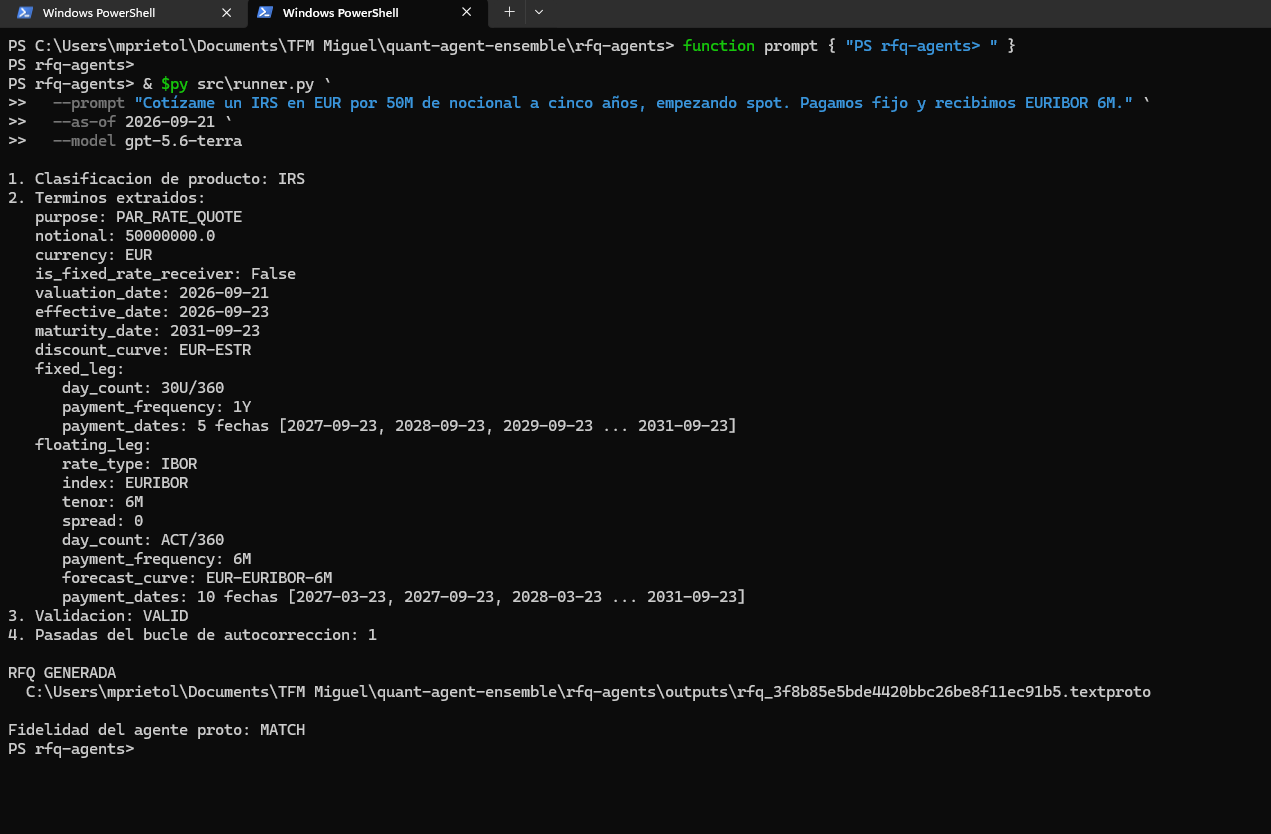
\includegraphics[width=\textwidth,keepaspectratio]{ejecucion_completa_rfq.png}
    \caption[Ejecución completa de una petición de RFQ]{Ejecución real desde una petición en lenguaje natural hasta la generación de la RFQ}
    \label{fig:ejecucion_completa_rfq}
    \floatfoot{Fuente: elaboración propia a partir de una ejecución real del sistema.}
\end{figure}

Para una cotización EUR a cinco años, el resultado contiene \texttt{purpose: PAR\_RATE\_QUOTE}, omite el tipo fijo y conserva el nocional, la dirección, las fechas, las curvas y ambas patas. La ausencia del tipo no es un error: representa la incógnita que resolvería el motor de valoración.

La ejecución crea dos archivos vinculados mediante el mismo identificador: un informe de validación y la \textit{RFQ} en \textit{textproto}. Si la petición es inválida, solo se conserva el informe; si el producto no está soportado, el flujo termina antes de crear ambos archivos.

\section{Reproducibilidad y repositorio}
\label{sec:reproducibilidad_repositorio}

El código, las instrucciones, el esquema, los casos y las bases archivadas se conservan en el repositorio público:

\begin{center}
\url{https://github.com/ProgramadorMiguel/quant-agent-ensemble}
\end{center}

La reproducción del entorno se apoya en cinco elementos: dependencias bloqueadas, instrucciones y esquema versionados, fecha de referencia explícita, casos comprobados de forma determinista y bases de datos archivadas. Las credenciales se documentan mediante \texttt{.env.example}, pero sus valores permanecen fuera del repositorio.

Antes de una tanda se ejecutan dos controles:

\begin{lstlisting}[
    language=bash,
    caption={Comprobaciones previas a la evaluación},
    label={cod:comprobaciones_reproducibilidad}
]
python tools/check_cases.py
python -m pytest -q
\end{lstlisting}

\texttt{check\_cases.py} analiza las 18 referencias estructuradas y verifica la etiqueta de los cinco productos no soportados. La batería de \texttt{pytest} contiene 84 pruebas sobre esquema, mapeo, convenciones, validación, autocorrección, métricas, costes y proveedores. Las rutas con reintentos y errores externos se prueban con clientes simulados.

La Figura~\ref{fig:pruebas_reproducibilidad} aporta evidencia de ambos controles: los 23 casos resultan coherentes con su familia y las 84 pruebas terminan correctamente.

\begin{figure}[H]
    \centering
    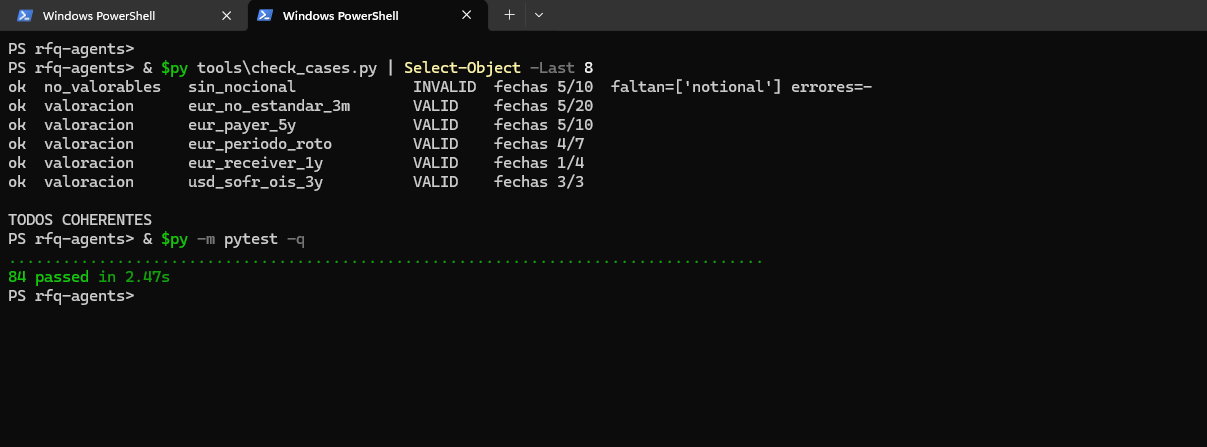
\includegraphics[width=\textwidth,keepaspectratio]{pruebas_reproducibilidad.png}
    \caption[Comprobación de las pruebas y los casos de referencia]{Comprobación de los 23 casos de referencia y ejecución de las 84 pruebas automatizadas}
    \label{fig:pruebas_reproducibilidad}
    \floatfoot{Fuente: elaboración propia a partir de una ejecución real del sistema.}
\end{figure}

Cada tanda recibe un \texttt{batch\_id}. Cada llamada registra además el proveedor, el modelo, el agente, la petición, la respuesta o error, una huella de las instrucciones, tokens, caché, latencia y coste. Cuando una tanda se utiliza como evidencia, su base se archiva en \texttt{evaluation/results/}. Los tokens permiten recalcular costes sin repetir llamadas si se corrige una tarifa.

La fecha de referencia se fija mediante \texttt{--as-of} para que expresiones como \textit{spot}, «el próximo lunes» o \texttt{2Y1Y} produzcan fechas comparables. La temperatura no puede fijarse en los modelos evaluados, por lo que reproducir la configuración no garantiza una respuesta idéntica. La reproducibilidad del trabajo consiste en conservar qué se ejecutó, bajo qué condiciones y qué respuesta produjo, no en atribuir determinismo a los proveedores.
